% !Mode:: "TeX:UTF-8"
\chapter{Visual Odometry: Part II}
\label{cpt:vo2}
\label{cpt:8}
\begin{mdframed}  
	\textbf{Goal of Study}
	\begin{enumerate}[labelindent=0em,leftmargin=1.5em]
		\item Understand the principle of optical flow to track feature points.
		\item Understand how the direct method estimates the camera pose.
		\item Use g2o for direct method.
	\end{enumerate}
\end{mdframed}

Different from feature point method, direct method is another main stream of visual odometry. Despite that it has not yet become the mainstream of VO, after recent years of development, the direct method can compete with feature point method to some extent. In this chapter, we will introduce the principle of the direct method and implement its core part.

\newpage
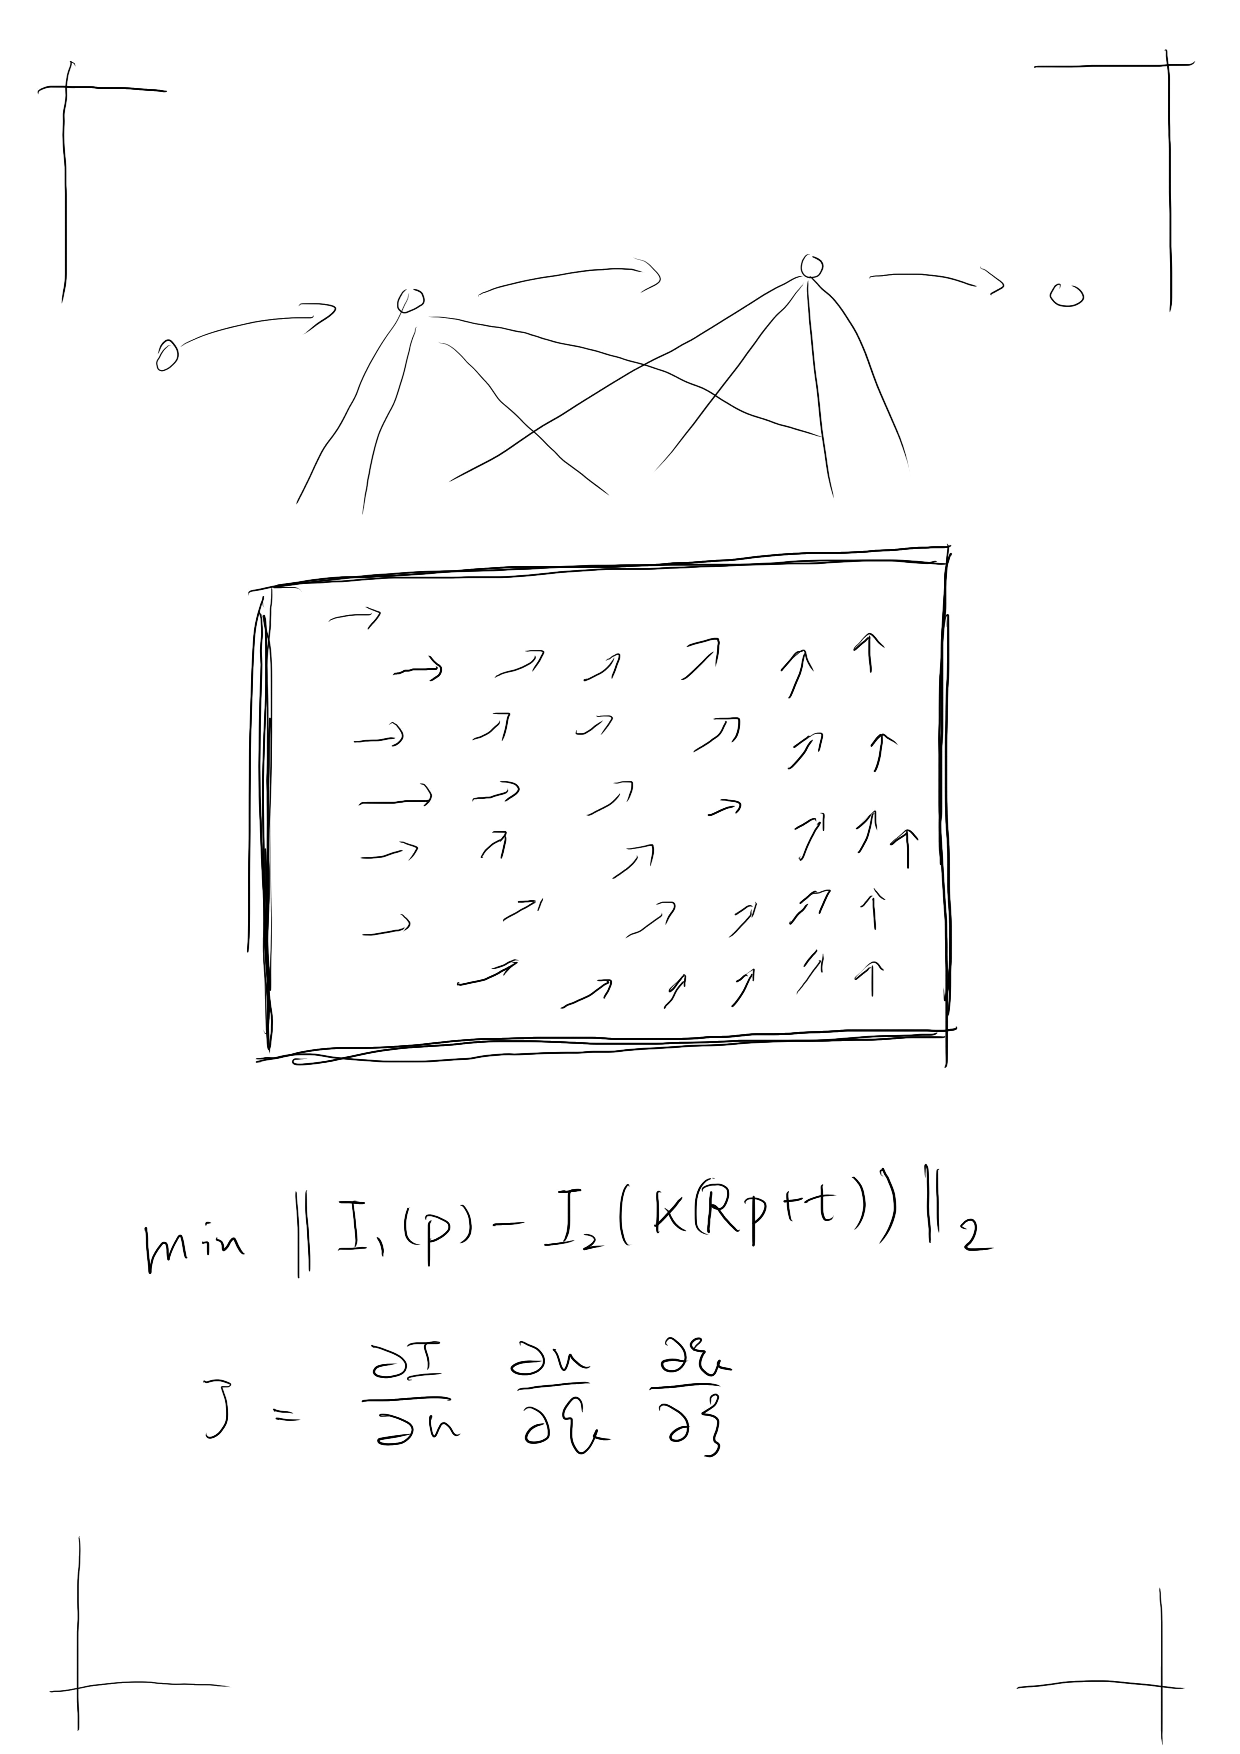
\includepdf{resources/other/ch8.pdf}

\newpage
\section{Origin of the direct method}
In the last chapter, we introduced using feature points to estimate camera motion. Although the feature point method plays a key role in visual odometry, researchers still believe that it has at least the following shortcomings:

\begin{enumerate}
	\item The extraction of key points and the calculation of descriptors are very time-consuming. In practice, SIFT currently cannot be calculated in real time on the CPU, and ORB also requires nearly 20ms of calculation. If the entire SLAM runs at a speed of 30 milliseconds per frame, more than half of the time will be spent on feature points calculation.

	\item When using feature points, all information except feature points is ignored. An image has hundreds of thousands of pixels, but only a few hundred feature points. Using only feature points discards most of the \textbf{possibly useful} image information. 
	
	\item The camera sometimes moves to places \textbf{lack of feature}, where there is often no obvious texture information. For example, sometimes we will face a white wall or an empty corridor. The number of feature points in these scenes will be significantly reduced, and we may not find enough matching points to calculate camera motion.。
\end{enumerate}

Now we see that there are indeed some problems with using feature points. Is there any way to overcome these shortcomings? We have the following ideas:

\begin{itemize}
	\item Keep feature points, but discard their descriptors. At the same time, use \textbf{Optical Flow} to track the motion of feature points. This can avoid the time brought by the calculation and matching of the descriptor, and the time spent on calculating optical flow itself is less than the descriptor calculation and matching.
	\item Only calculate key points, not descriptors. At the same time, use \textbf{Direct Method} to calculate the position of the feature point in the image at the next timestamp. This can also save the time spent on the calculation of the descriptor as well as the the calculation of optical flow.	
\end{itemize}

The first method still uses feature points, but substitutes the descriptor matching with optical flow tracking, and still uses epipolar geometry, PnP or ICP algorithms to estimate camera motion. This still requires that the extracted keypoints are distinguishable, that is, we need to extract the corner points. In the direct method, we will estimate the camera motion and the projection of the points at the same time according to the \textbf{pixel gray information} of the image, and the extracted points to be corner points is not longer a hard prerequisite. As you will see later, they can even be randomly selected points.

When using the feature point method to estimate camera motion, we regard feature points as fixed points in three-dimensional space. According to their projection position in the camera, the camera motion is optimized by \textbf{minimize reprojection error}. In this process, we need to know exactly the pixel position of the spatial point after the projection of the two cameras-this is why we need to match or track the features. Meanwhile, computing and matching features requires a lot of computation. In contrast, in the direct method, we do not need to know the correspondence between points in advance, but find it by minimizing \textbf{Photometric error}.

We will focus on the direct method in this chapter. It is to overcome the shortcomings of the feature point method listed above. The direct method estimates the camera motion based on the brightness information of the pixels, and can completely eliminate the calculation of keypoints and descriptors. Therefore, it not only saves the calculation time of features, but also solves the problems caused by lacking features. As long as there are brightness changes in the scene (it can be a gradual change without forming a local image gradient), the direct method will work. According to the number of pixels used, the direct method can be categorized into sparse, semi-dense and dense. Compared with the feature point method that can only reconstruct sparse feature points (sparse map), the direct method also has the capability to restore semi-dense or dense structures.

Historically, there were also early uses of the direct method \textsuperscript{\cite{Silveira2008}}. With the emergence of some open source projects that use the direct method, such as SVO\textsuperscript{\cite{Forster2014}}, LSD-SLAM\textsuperscript{\cite{Engel2014}}, DSO\textsuperscript{\cite{Engel2016}}, etc. Direct method became a more and more important part of the visual odometry.

\section{2D Optical Flow}
Direct method was inspired by the optical flow. They are similar and use the same assumptions. Optical flow describes the motion of pixels in the image, and the direct method is accompanied by a camera motion model. Before the direct method, we will introduce optical flow first.

Optical flow is a method of describing the movement of pixels between images, as shown in \autoref{fig:LK}~. The same pixel will move in the image over time, and we want to track its movement. The calculation of motion of a portion of pixels is called \textbf{sparse optical flow}, and the calculation of all pixels in an image is called \textbf{dense optical flow}. A well-known sparse optical flow method is called Lucas-Kanade optical flow \textsuperscript{\cite{Lucas1981}}. It can be used to track the position of feature points in SLAM. Dense optical flow is represented by Horn-Schunck optical flow \textsuperscript{\cite{Horn1981}}. This section mainly introduces Lucas-Kanade optical flow, also known as LK optical flow.

\begin{figure}[!htp]
	\centering
	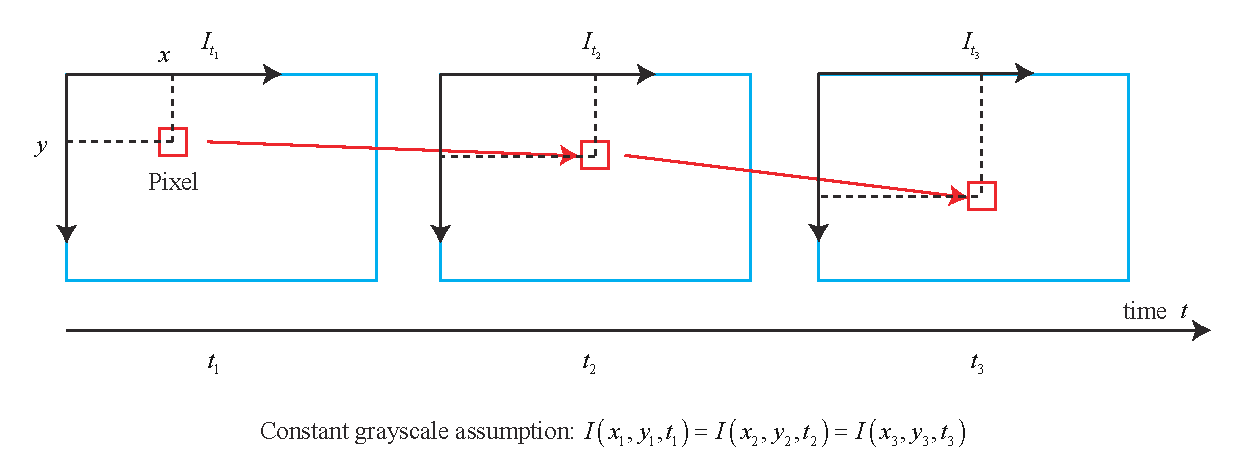
\includegraphics[width=1.0\linewidth]{vo2/opticalFlow}
	\caption{workflow of LK method}
	\label{fig:LK}
\end{figure}

\subsection*{Lucas-Kanade optical flow}
In the LK optical flow, we think that the image from the camera changes over time. The image can be regarded as a function of time $\mathbf{I}(t)$. Then, for a pixel at $(x,y)$ at time $t$, its grayscale can be written as
\[
\mathbf{I}(x,y,t).
\]
In this way, the image is regarded as a function of position and time, and its range is the grayscale of the pixels in the image. Now consider a fixed point in space, its pixel coordinates at time $t$ are $x,y$. Due to the movement of the camera, its image coordinates will change. We want to estimate the position of this space point in the image at other times. How to estimate it? Here we will introduce the basic assumptions of the optical flow method.

\textbf{Constant Brightness}:The pixel grayvalue of the same space point is constant in each image.

For the pixel at $(x,y)$ at time $t$, suppose it moves to $(x+\mathrm{d}x, y+\mathrm{d}y)$ at time $t+\mathrm{d}t$. Since the grayscale is unchanged, we have:
\begin{equation} 
\mathbf{I}(x+\mathrm{d}x, y+\mathrm{d}y, t+\mathrm{d}t) = \mathbf{I} (x,y,t).
\end{equation}

Note that in the most of time in practice the assumption of constant brightness is not true. In fact, due to the different materials of the objects, the pixels will have highlights and shadows; sometimes, the camera will automatically adjust its exposure parameters to make the overall image brighter or darker. At these times, the assumption of constant brightness is invalid, so the result of optical flow is not necessarily reliable. However, on the other hand, all algorithms work under certain assumptions. If we do not make any assumptions, we cannot design practical algorithms. So, let us consider this assumption to be true for now and see how to calculate the motion of the pixels.

Carry out Taylor expansion on the left side and only keep the first-order term, we have:
\begin{equation}
\mathbf{I} \left( {x + \mathrm{d}x,y + \mathrm{d}y,t + \mathrm{d}t} \right) \approx \mathbf{I} \left( {x,y,t} \right) + \frac{{\partial \mathbf{I} }}{{\partial x}}\mathrm{d}x + \frac{{\partial \mathbf{I}}}{{\partial y}}\mathrm{d}y + \frac{{\partial \mathbf{I}}}{{\partial t}}\mathrm{d}t.
\end{equation}

Because we assume that the brightness does not change, the brightness at the next timestamp is equal to the current one, thus:
\begin{equation}
 \frac{{\partial \mathbf{I} }}{{\partial x}}\mathrm{d}x + \frac{{\partial \mathbf{I}}}{{\partial y}}\mathrm{d}y + \frac{{\partial \mathbf{I}}}{{\partial t}}\mathrm{d}t = 0.
\end{equation}

Divide both sides by $\mathrm{d}t$:
\begin{equation}\label{key}
 \frac{{\partial \mathbf{I} }}{{\partial x}} \frac{\mathrm{d}x}{\mathrm{d}t} + \frac{{\partial \mathbf{I}}}{{\partial y}} \frac{\mathrm{d}y}{\mathrm{d}t} =- \frac{{\partial \mathbf{I}}}{{\partial t}}.
\end{equation}

Where $\mathrm{d}x / \mathrm{d}t$ is the speed of the pixel on the $x$ axis, and $\mathrm{d}y/\mathrm{d}t$ is the speed on the $y$ axis, denoting them as $u,v$. At the same time, $\partial \mathbf{I}/{\partial x}$ is the gradient of the image in the $x$ direction at this point, and the other is the gradient in the $y$ direction, denoted as $\mathbf{I} _x, \mathbf{I}_y$. Denote the change of the image brightness with respect to time as $\mathbf{I}_t$. They can be written in a matrix form as:
\begin{equation}
\left[ {\begin{array}{*{20}{c}}
	{{ \mathbf{I}_x}}&{{ \mathbf{I}_y}}
	\end{array}} \right]\left[ \begin{array}{l}
u\\
v
\end{array} \right] =  - {\mathbf{I}_t}.
\end{equation}

What we want is to calculate the motion $u,v$ of the pixel, but this formula is a linear equation with two variables, and we cannot find $u,v$ by itself. Therefore, additional constraints are needed to calculate $u,v$. In LK optical flow, we assume \textbf{pixels in a certain window have the same motion}.

Consider a window of size $w \times w$, which contains $w^2$ pixels. Since the pixels in this window are assumed to have the same motion, we have a total of $w^2$ equations:
\begin{equation}
\left[ {\begin{array}{*{20}{c}}
	{{ \mathbf{I}_x}}&{{ \mathbf{I}_y}}
	\end{array}} \right]_k
\left[ \begin{array}{l}
u\\
v
\end{array} \right] =  - {\mathbf{I}_t}_k, \quad k=1, \ldots, w^2.
\end{equation}

Stacking them:
\begin{equation}
\mathbf{A} = \left[ {\begin{array}{*{20}{c}}
	{{{\left[ {{\mathbf{I}_x},{\mathbf{I}_y}} \right]}_1}}\\
	\vdots \\
	{{{\left[ {{\mathbf{I}_x},{\mathbf{I}_y}} \right]}_k}}
	\end{array}} \right],\mathbf{b} = \left[ {\begin{array}{*{20}{c}}
	{{ \mathbf{I}_{t1}}}\\
	\vdots \\
	{{ \mathbf{I}_{tk}}}
	\end{array}} \right].
\end{equation}

The whole equation is:
\begin{equation}
\mathbf{A}\left[ \begin{array}{l}
u\\
v
\end{array} \right] =  - \mathbf{b}.
\end{equation}

This is an overdetermined linear equation about $u,v$. And we can find its least square solution.
\begin{equation}
{\left[ \begin{array}{l}
	u\\
	v
	\end{array} \right]^*} = -{\left( {{ \mathbf{A}^\mathrm{T}}\mathbf{A}} \right)^{ - 1}}{ \mathbf{A}^\mathrm{T}}\mathbf{b}.
\end{equation}

In this way, the speed $u,v$ of pixels between images is obtained. When $t$ takes discrete moments instead of continuous time, we can estimate the position of a block of pixels in several images. Since the pixel gradient is only valid locally, if one iteration does not produce a reasonable result, we will iterate this calculation several times. In SLAM, LK optical flow is often used to track the motion of corner points. We can have a deeper understanding of it through the program.

\section{Practice: LK Optical Flow}
\label{sec:LKFlow}
%\subsection{Use TUM Dataset online}
%The following demonstrates how to use the optical flow method provided by OpenCV to track feature points. As in the previous section, we have prepared several dataset images, which are stored in the data/ folder. They come from the public RGB-D dataset (TUM dataset) \footnote{see \url{http://vision.in.tum.de/data/datasets/rgbd-dataset/download} provided by the Technical University of Munich}. It contains many RGB-D videos, which can be used as experimental data for RGB-D or monocular SLAM. It also provides an accurate trajectory measured by the motion capture system, which can be used as a standard trajectory to calibrate the SLAM system. Because the data set is relatively large, we did not put it on GitHub, please go to the dataset homepage to retrieve the corresponding data. Part of the images in the "freburg1\_desk" data set are used in this program. Readers can find its download link on the TUM dataset homepage. Or, you can directly use the part of it provided on GitHub repo.
%
%Our data is located under data/ in the directory of this chapter as a compressed package (data.tar.gz). Since the TUM data set is collected from the actual environment, it is necessary to explain its data format (data sets generally have their own defined format). After unzipping, you will see the following files:
%
%\begin{enumerate}
% 	\item rgb.txt and depth.txt record the collection time of each file and the corresponding file name.
% 	\item rgb/ and depth/ directories store the captured PNG format image files. The color image is 8-bit 3 channels, and the depth map is 16-bit single-channel image. The file name is the collection time.
%	
% 	\item groundtruth.txt is the camera pose collected by the external motion capture system, the format is
% 	\[
% 	(\mathrm{time}, t_x, t_y, t_z, q_x, q_y, q_z, q_w),
% 	\]
% 	We can treat it as a standard trajectory (ground truth).
%\end{enumerate}
%
%Please note that the collection of color image, depth image and standard trajectory are all independent, and the trajectory collection frequency is much higher than that of the image. Before using the data, it is necessary to align the data in time according to the collection time in order to pair the color map and the depth map. In principle, we can regard data whose collection time is close to a threshold as a pair of images. And regard the pose at a similar time as the true collection position of the image. TUM provides a Python script "associate.py" (or use slambook/tools/associate.py) to help us accomplish this. Please put this file in the data set directory and run:
%\begin{lstlisting}[language=sh]
%python associate.py rgb.txt depth.txt> associate.txt
%\end{lstlisting}
%
%This script will match according to the collection time in the two input files, and finally output to the file associate.txt. The output file contains the time and file name information of the two images after pairing, which can be used as the source for subsequent processing. In addition, the TUM data set also provides tools for comparing estimated trajectories with standard trajectories. We will introduce them when they are used.
\subsection{Use LK optical flow}
In the practice, we will use several sample images to track their feature points with OpenCV optical flow. At the same time, we will also manually implement a LK optical flow for a comprehensive understanding. We use two sample images from the Euroc dataset, extract the corner points in the first image, and then use optical flow to track their position in the second image. First, let's use the LK optical flow in OpenCV:

\begin{lstlisting}[language=c++,caption=slambook2/ch8/optical_flow.cpp (snippet))]
// use opencv's flow for validation
vector<Point2f> pt1, pt2;
for (auto &kp: kp1) pt1.push_back(kp.pt);
vector<uchar> status;
vector<float> error;
cv::calcOpticalFlowPyrLK(img1, img2, pt1, pt2, status, error);
\end{lstlisting}

The optical flow in OpenCV is very simple to use. You only need to call the cv::calcOpticalFlowPyrLK function, provide two images and the corresponding feature points, you can get the tracked points, as well as the status and error of each point. We can determine whether the corresponding point is tracked correctly according to whether the status variable is 1. This function also has some optional parameters, but in the demonstration we only use the default parameters. We omit other codes that mention features and draw results here, which have been shown in the previous code snippet.

\subsection{Implement optical flow with Gauss Newton method}
\subsubsection{Single-layer optical flow}
Optical flow can also be seen as an optimization problem: by minimizing the grayscale error, the optimal pixel shift is estimated. Therefore, similar to those various Gauss-Newton methods previously implemented, we now also implement an optical flow based on the Gauss-Newton method.

\begin{lstlisting}[language=c++,caption=slambook2/ch8/optical_flow.cpp (snippet))]
class OpticalFlowTracker {
public:
	OpticalFlowTracker(
		const Mat &img1_,
		const Mat &img2_,
		const vector<KeyPoint> &kp1_,
		vector<KeyPoint> &kp2_,
		vector<bool> &success_,
		bool inverse_ = true, bool has_initial_ = false) :
		img1(img1_), img2(img2_), kp1(kp1_), kp2(kp2_), success(success_), inverse(inverse_),
		has_initial(has_initial_) {}
	
	void calculateOpticalFlow(const Range &range);

private:
	const Mat &img1;
	const Mat &img2;
	const vector<KeyPoint> &kp1;
	vector<KeyPoint> &kp2;
	vector<bool> &success;
	bool inverse = true;
	bool has_initial = false;
};

void OpticalFlowSingleLevel(
	const Mat &img1,
	const Mat &img2,
	const vector<KeyPoint> &kp1,
	vector<KeyPoint> &kp2,
	vector<bool> &success,
	bool inverse, bool has_initial) {
	kp2.resize(kp1.size());
	success.resize(kp1.size());
	OpticalFlowTracker tracker(img1, img2, kp1, kp2, success, inverse, has_initial);
	parallel_for_(Range(0, kp1.size()),
		std::bind(&OpticalFlowTracker::calculateOpticalFlow, &tracker, placeholders::_1));
}

void OpticalFlowTracker::calculateOpticalFlow(const Range &range) {
	// parameters
	int half_patch_size = 4;
	int iterations = 10;
	for (size_t i = range.start; i < range.end; i++) {
		auto kp = kp1[i];
		double dx = 0, dy = 0; // dx,dy need to be estimated
		if (has_initial) {
			dx = kp2[i].pt.x - kp.pt.x;
			dy = kp2[i].pt.y - kp.pt.y;
		}
		
		double cost = 0, lastCost = 0;
		bool succ = true; // indicate if this point succeeded
		
		// Gauss-Newton iterations
		Eigen::Matrix2d H = Eigen::Matrix2d::Zero();    // hessian
		Eigen::Vector2d b = Eigen::Vector2d::Zero();    // bias
		Eigen::Vector2d J;  // jacobian
		for (int iter = 0; iter < iterations; iter++) {
			if (inverse == false) {
				H = Eigen::Matrix2d::Zero();
				b = Eigen::Vector2d::Zero();
			} else {
				// only reset b
				b = Eigen::Vector2d::Zero();
			}
			
			cost = 0;
			
			// compute cost and jacobian
			for (int x = -half_patch_size; x < half_patch_size; x++)
			for (int y = -half_patch_size; y < half_patch_size; y++) {
				double error = GetPixelValue(img1, kp.pt.x + x, kp.pt.y + y) -
					GetPixelValue(img2, kp.pt.x + x + dx, kp.pt.y + y + dy);;  // Jacobian
				if (inverse == false) {
					J = -1.0 * Eigen::Vector2d(
						0.5 * (GetPixelValue(img2, kp.pt.x + dx + x + 1, kp.pt.y + dy + y) -
							GetPixelValue(img2, kp.pt.x + dx + x - 1, kp.pt.y + dy + y)),
						0.5 * (GetPixelValue(img2, kp.pt.x + dx + x, kp.pt.y + dy + y + 1) -
							GetPixelValue(img2, kp.pt.x + dx + x, kp.pt.y + dy + y - 1))
					);
				} else if (iter == 0) {
					// in inverse mode, J keeps same for all iterations
					// NOTE this J does not change when dx, dy is updated, so we can store it and only compute error
					J = -1.0 * Eigen::Vector2d(
						0.5 * (GetPixelValue(img1, kp.pt.x + x + 1, kp.pt.y + y) -
							GetPixelValue(img1, kp.pt.x + x - 1, kp.pt.y + y)),
						0.5 * (GetPixelValue(img1, kp.pt.x + x, kp.pt.y + y + 1) -
							GetPixelValue(img1, kp.pt.x + x, kp.pt.y + y - 1))
					);
				}
				// compute H, b and set cost;
				b += -error * J;
				cost += error * error;
				if (inverse == false || iter == 0) {
					// also update H
					H += J * J.transpose();
				}
			}
			
			// compute update
			Eigen::Vector2d update = H.ldlt().solve(b);
			
			if (std::isnan(update[0])) {
				// sometimes occurred when we have a black or white patch and H is irreversible
				cout << "update is nan" << endl;
				succ = false;
				break;
			}
			
			if (iter > 0 && cost > lastCost) {
				break;
			}
			
			// update dx, dy
			dx += update[0];
			dy += update[1];
			lastCost = cost;
			succ = true;
			
			if (update.norm() < 1e-2) {
				// converge
				break;
			}
		}
		
		success[i] = succ;
		
		// set kp2
		kp2[i].pt = kp.pt + Point2f(dx, dy);
	}
}
\end{lstlisting}

We have implemented a single-layer optical flow function in the OpticalFlowSingleLevel function, in which cv::parallel\_for\_ is called in parallel to call OpticalFlowTracker::calculateOpticalFlow, which calculates the optical flow of feature points within a specified range. This parallel for loop is internally implemented by the Intel tbb library. We only need to define the function body according to its interface, and then pass the function to it as a std::function object.

In the implementation of calculateOpticalFlow, we solve such a problem:
\begin{equation}
\mathop {\min }\limits_{\Delta x,\Delta y} \left\| {{\mathbf{I}_1}\left( {x,y} \right) - {\mathbf{I}_2}\left( {x + \Delta x,y + \Delta y} \right)} \right\|_2^2.
\end{equation}
Therefore, the residual is the part inside the brackets, and the corresponding Jacobian is the gradient of the second image at $x + \Delta x,y + \Delta y$. In addition, according to \cite{Baker2004}, the gradient can also be replaced by the gradient $\mathbf{I}_1 (x,y)$ of the first image. This is called \textbf{Inverse} optical flow method. In inverse optical flow, the gradient of $\mathbf{I}_1 (x,y)$ remains unchanged, so we can use the result calculated in the first iteration in the subsequent iterations. When the Jacobian remains unchanged, the $\mathbf{H}$ matrix is unchanged, and only the residual is calculated for each iteration, which can save a lot of calculation.

\subsubsection{Multi-layer optical flow}
Since we write optical flow as an optimization problem, we must assume that the initial value of optimization is close to the optimal value to ensure the convergence of the algorithm. Therefore, if the camera moves faster and the difference between the two images is obvious, the single-layer image optical flow method can be easily stuck at a local minimum. While it can be resolved to some extent by image pyramids.

\begin{figure}[!htp]
	\centering
	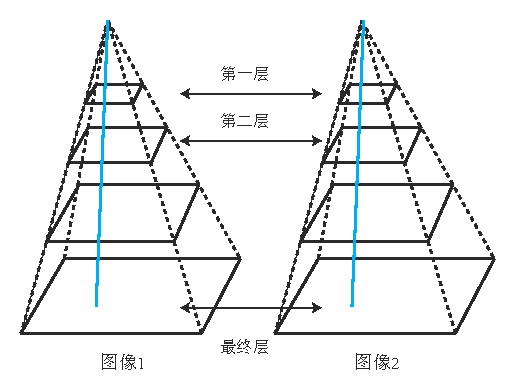
\includegraphics[width=.7\linewidth]{vo2/image-pyramid}
	\caption{Image pyramid and coarse-to-fine process.}
	\label{fig:image-pyramid}
\end{figure}

Image pyramid refers to scaling the image to get samples in different resolutions, as shown in \autoref{fig:image-pyramid}. The original image is used as the bottom layer of the pyramid. Every time one layer goes up, the lower layer image is scaled to a certain magnification, and then a pyramid is obtained. When calculating the optical flow, start from the top layer image, and then use the tracking result of the previous layer as the initial value of the optical flow of the next layer. Since the upper layer image is relatively rough, this process is also called \textbf{coarse-to-fine} optical flow, which is also the usual process of optical flow in practice.

The advantage of going from coarse to fine is that when the pixel motion of the original image is large, the motion is still within a small range from the image at the top of the pyramid. For example, if the feature points of the original image move by 20 pixels, it is easy for the optimization to be trapped in the minimum value due to the non-convexity of the image. But now suppose there is a pyramid with a zoom magnification of 0.5 times, then in the upper two layers of images, the pixel movement is only 5 pixels, and the result is obviously better than directly optimizing on the original image.

We have implemented multi-layer optical flow in the program, the code is as follows:
\begin{lstlisting}[language=c++,caption=slambook2/ch8/optical_flow.cpp (snippet)]
void OpticalFlowMultiLevel(
	const Mat &img1,
	const Mat &img2,
	const vector<KeyPoint> &kp1,
	vector<KeyPoint> &kp2,
	vector<bool> &success,
	bool inverse) {
	
	// parameters
	int pyramids = 4;
	double pyramid_scale = 0.5;
	double scales[] = {1.0, 0.5, 0.25, 0.125};
	
	// create pyramids
	vector<Mat> pyr1, pyr2; // image pyramids
	for (int i = 0; i < pyramids; i++) {
		if (i == 0) {
			pyr1.push_back(img1);
			pyr2.push_back(img2);
		} else {
			Mat img1_pyr, img2_pyr;
			cv::resize(pyr1[i - 1], img1_pyr,
			cv::Size(pyr1[i - 1].cols * pyramid_scale, pyr1[i - 1].rows * pyramid_scale));
			cv::resize(pyr2[i - 1], img2_pyr,
			cv::Size(pyr2[i - 1].cols * pyramid_scale, pyr2[i - 1].rows * pyramid_scale));
			pyr1.push_back(img1_pyr);
			pyr2.push_back(img2_pyr);
		}
	}

	// coarse-to-fine LK tracking in pyramids
	vector<KeyPoint> kp1_pyr, kp2_pyr;
	for (auto &kp:kp1) {
		auto kp_top = kp;
		kp_top.pt *= scales[pyramids - 1];
		kp1_pyr.push_back(kp_top);
		kp2_pyr.push_back(kp_top);
	}
	
	for (int level = pyramids - 1; level >= 0; level--) {
		// from coarse to fine
		success.clear();
		OpticalFlowSingleLevel(pyr1[level], pyr2[level], kp1_pyr, kp2_pyr, success, inverse, true);
		
		if (level > 0) {
			for (auto &kp: kp1_pyr)
			kp.pt /= pyramid_scale;
			for (auto &kp: kp2_pyr)
			kp.pt /= pyramid_scale;
		}
	}
	
	for (auto &kp: kp2_pyr)
		kp2.push_back(kp);
}
\end{lstlisting}

This code constructs a four-layer pyramid with a scaling rate of 0.5, and calls the single-layer optical flow function to achieve the multi-layer optical flow. In the main function, we tested the performance of OpenCV's optical flow, single-layer optical flow, and multi-layer optical flow on two images, and recorded their runtime:
\begin{lstlisting}[language=sh,caption=终端输入:]
./build/optical_flow
build pyramid time: 0.000150349
track pyr 3 cost time: 0.000304633
track pyr 2 cost time: 0.000392889
track pyr 1 cost time: 0.000382347
track pyr 0 cost time: 0.000375099
optical flow by gauss-newton: 0.00189268
optical flow by opencv: 0.00220134
\end{lstlisting}
In terms of runtime, the multi-layer optical flow method takes roughly the same time as OpenCV. Since the performance of the parallelized program varies from run to run, these numbers will not be exactly the same on the reader's machine. For the result of optical flow, see \autoref{fig:optical-flow-result}. It can be seen that the multi-layer optical flow has the same effect as OpenCV, and the single-layer optical flow performs obviously worser than the multi-layer optical flow.

\begin{figure}[!htp]
	\centering
	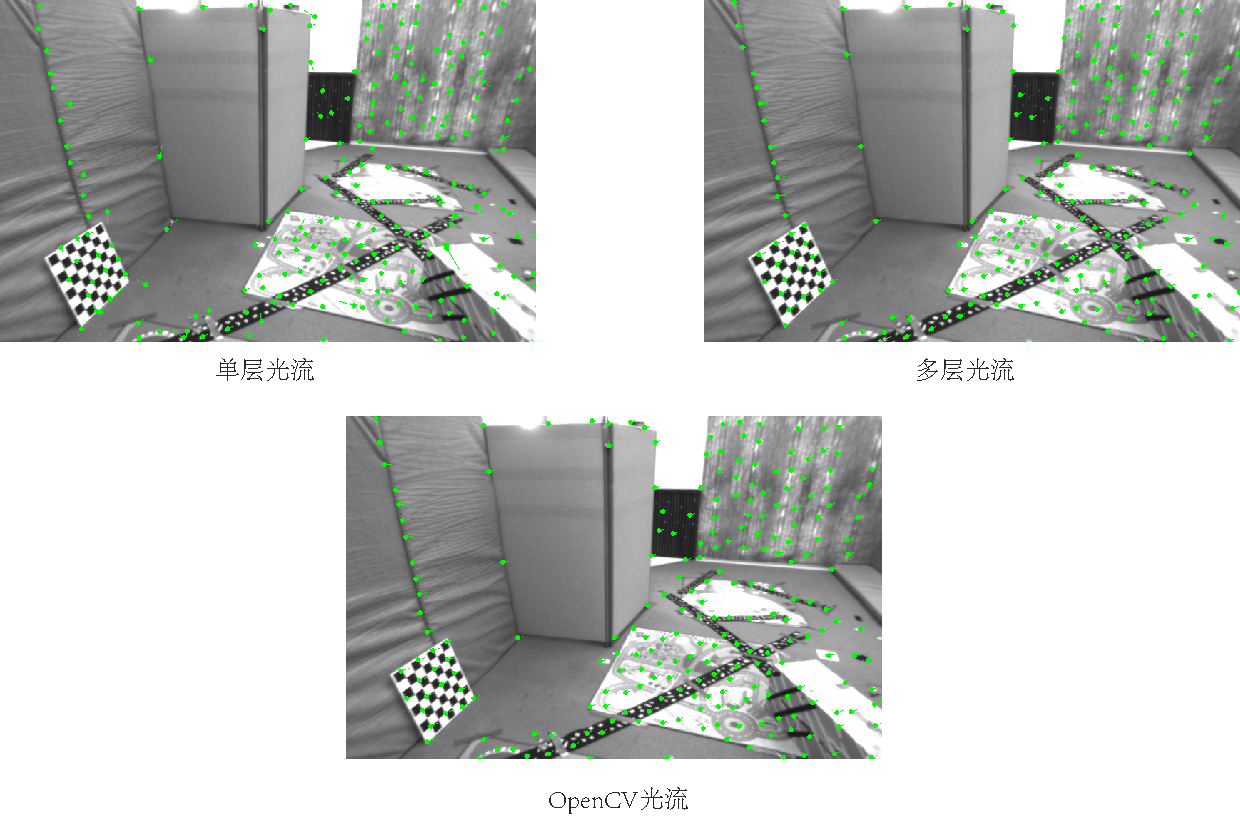
\includegraphics[width=.85\linewidth]{vo2/optical-flow}
	\caption{Comparison of the results of various optical flows}
	\label{fig:optical-flow-result}
\end{figure}

\subsection{Summary of optical flow practice}
We see that LK optical flow can directly obtain the corresponding relationship of feature points. This correspondence is like the matching of descriptors, except that optical flow requires higher image continuity and light stability. We can use PnP, ICP, or epipolar geometry to estimate the camera motion through the feature points tracked by optical flow. These methods were introduced in the previous lecture and will not be discussed here.

In terms of runtime, it extracts about 230 feature points in the experiment. OpenCV and multi-layer optical flow need about 2 milliseconds to complete the tracking (the CPU I use is Intel I7-8550U), which is quite fast. If we use keypoints like FAST, then the entire optical flow calculation can be done in about 5 milliseconds, which is very fast compared to feature matching. However, if the position of the corner point is not good, the optical flow is also easy to be lost or give wrong results, which requires the subsequent algorithm to have a certain outlier removal mechanism, we leave the relevant discussion to the later chapter.

In a nutshell, the optical flow method can accelerate the visual odometry calculation method based on feature points by avoiding the process of calculating and matching descriptors, but requires smoother camera movement (or higher collection frequency).

\section{Direct Method}
Next, let's discuss the direct method, which is somehow similar to the optical flow method. We first introduce the principle of the direct method, and then implement the direct method.

\subsection{Derivation of the direct method}
In the optical flow, we will first track the location of feature points, and then determine the camera's movement based on these locations. Then, such a two-step plan is difficult to guarantee the overall optimality. We can ask, can we adjust the result of the previous step in the latter step? For example, if I think that the camera has turned 15 degrees to the right, can the optical flow use this 15-degree motion as the initial value to adjust the calculation of the optical flow? This idea is reflected in the direct method.

As shown in \autoref{fig:directMethod}~, consider a spatial point $P$ and camera at two timestamps. The world coordinates of $P$ are $[X,Y,Z]$, and the pixel coordinates of its imaging on two cameras are $\mathbf{p}_1, \mathbf{p}_2$.

\begin{figure}[!htp]
	\centering
	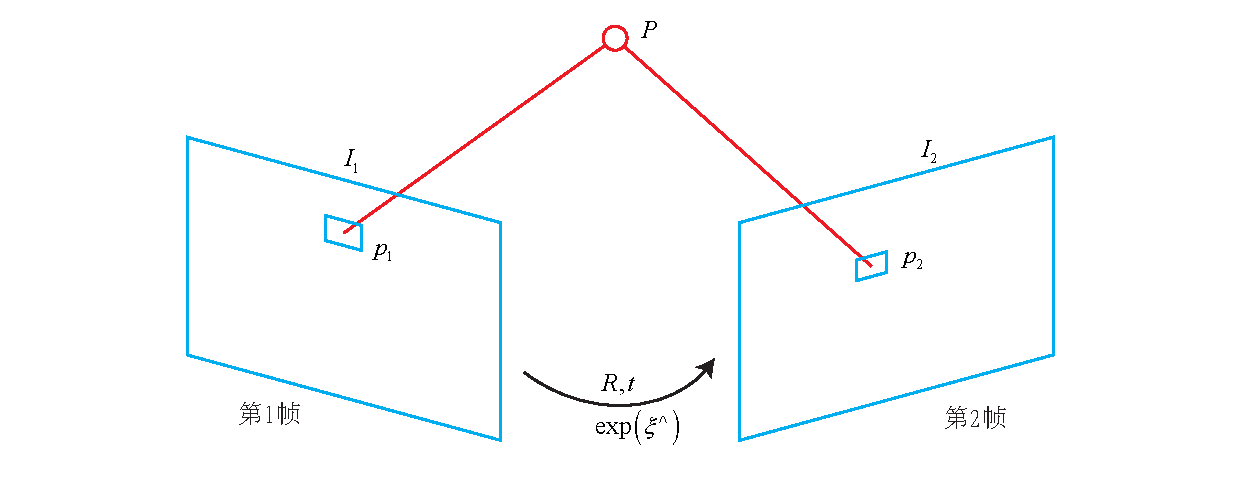
\includegraphics[width=.85\linewidth]{vo2/directMethod}
	\caption{the direct method.}
	\label{fig:directMethod}
\end{figure}

Our goal is to find the relative pose transformation from the first camera to the second camera. We take the first camera as the frame of reference, and set the rotation and translation of the second camera as $\mathbf{R}, \mathbf{t}$ (corresponding to the Lie group as $\mathbf{T}$). At the same time, the internal parameters of the two cameras are the same, denoted as $\mathbf{K}$. Let's write down the complete projection equation:
\begin{align*}
{\mathbf{p}_1} &= {\left[ \begin{array}{l}
	u\\
	v\\
	1
	\end{array} \right]_1} = \frac{1}{Z_1} \mathbf{KP}, \\
{\mathbf{p}_2} &= {\left[ \begin{array}{l}
	u\\
	v\\
	1
	\end{array} \right]_2} = \frac{1}{Z_2} \mathbf{K}\left( {\mathbf{RP} +\mathbf{t}} \right) = \frac{1}{Z_2} \mathbf{K} \left(\mathbf{T}  \mathbf{P} \right)_{1:3}.
\end{align*}
Where $Z_1$ is the depth of $P$, and $Z_2$ is the depth of $P$ in the second camera frame, which is the third coordinate of $\mathbf{RP}+\mathbf{t}$ . Since $\mathbf{T}$ can only be multiplied with homogeneous coordinates, we need to take out the first 3 elements after multiplying. This is consistent with the content of \ref{cpt:5}.

Recall that in the feature point method, since we know the pixel positions of $\mathbf{p}_1, \mathbf{p}_2$ through matching descriptors, we can calculate the reprojection position. But in the direct method, since there is no feature matching, we have no way of knowing which $\mathbf{p}_2$ and $\mathbf{p}_1$ correspond to the same point. The idea of the direct method is to find the position of $\mathbf{p}_2$ according to the current camera pose estimation. But if the camera pose is not good enough, the appearance of $\mathbf{p}_2$ and $\mathbf{p}_1$ will be significantly different. Therefore, in order to reduce this difference, we optimize the pose of the camera to find $\mathbf{p}_2$ that is more similar to $\mathbf{p}_1$. This can also be done by solving an optimization problem, but at this time it is not to minimize the reprojection error, but to minimize the \textbf{Photometric Error}, which is the brightness error of the two pixels of $P$:
\begin{equation}
e = {\mathbf{I}_1}\left( {{\mathbf{p}_1}} \right) - {\mathbf{I}_2}\left( {{\mathbf{p}_2}} \right).
\end{equation}

Note that $e$ is a scalar here. Similarly, the optimization is with respect to the second norm of the error, taking the unweighted form for now, as:
\begin{equation}
\mathop {\min }\limits_{\mathbf{T}}  J\left( \mathbf{T}  \right) = \|e\|^2.
\end{equation}

The optimization is based on \textbf{constant brightness assumption}. We assume that the grayscale of a spatial point imaged at various viewing points is constant. If we have many (for example, $N$) space points $P_i$, then the whole camera pose estimation problem becomes
\begin{equation}
\mathop {\min }\limits_{\mathbf{T}}  J\left( \mathbf{T}  \right) = \sum\limits_{i = 1}^N {e_i^\mathrm{T}{e_i}}, \quad {e_i} = {\mathbf{I}_1}\left( {{\mathbf{p}_{1,i}}} \right) - {\mathbf{I}_2}\left( {{ \mathbf{p}_{2,i}}} \right).
\end{equation}

The variable to be optimized here is the camera pose $\mathbf{T}$, instead of the motion of each feature point in the optical flow. In order to solve this optimization problem, we are concerned about how the error $e$ changes with the camera pose $\mathbf{T}$, and we need to analyze their derivative relationship. First, define two intermediate variables:
\begin{align*}
\mathbf{q} &= \mathbf{T} \mathbf{P}, \\
\mathbf{u} &= \frac{1}{{{Z_2}}} \mathbf{K} \mathbf{q}.
\end{align*}
Here, $\mathbf{q}$ is the coordinates of $P$ in the second camera coordinate system, and $\mathbf{u}$ is its pixel coordinates. Obviously $\mathbf{q}$ is a function of $\mathbf{T}$, and $\mathbf{u}$ is a function of $\mathbf{q}$, and thus is also a function of $\mathbf{T}$. Consider the left perturbation model of Lie algebra, using the first-order Taylor expansion:
\begin{equation}
e(\mathbf{T})=\mathbf{I}_1(\mathbf{p}_{1})-\mathbf{I}_2(\mathbf{u}),
\end{equation}
所以:
\begin{equation}
\frac{\partial e}{\partial \mathbf{T}} = \frac{{\partial {\mathbf{I}_2}}}{{\partial \mathbf{u}}}\frac{{\partial \mathbf{u}}}{{\partial \mathbf{q}}}\frac{{\partial \mathbf{q}}}{{\partial \delta \mathbf{\xi} }}\delta \mathbf{\xi},
\end{equation}
Where $\delta \mathbf{\xi}$ is the left disturbance of $\mathbf{T}$. We see that the first derivative is divided into 3 terms due to the chain rule, and these 3 terms are easy to obtain:

\begin{enumerate}
	\item $ \partial \mathbf{I}_2 / \partial \mathbf{u} $ is the grayscale gradient at pixel $\mathbf{u}$.
	\item $ \partial \mathbf{u} / \partial \mathbf{q} $ is the derivative of the projection equation with respect to the three-dimensional point in the camera frame. Remember $\mathbf{q}=[X,Y,Z]^\mathrm{T}$, according to $\ref{cpt:7}$, the derivative is
	\begin{equation}
	\frac{{\partial \mathbf{u}}}{{\partial \mathbf{q}}} = \left[ {\begin{array}{*{20}{c}}
		{\frac{{\partial u}}{{\partial X}}}&{\frac{{\partial u}}{{\partial Y}}}&{\frac{{\partial u}}{{\partial Z}}}\\
		{\frac{{\partial v}}{{\partial X}}}&{\frac{{\partial v}}{{\partial Y}}}&{\frac{{\partial v}}{{\partial Z}}}
		\end{array}} \right] = \left[ {\begin{array}{*{20}{c}}
		{\frac{{{f_x}}}{{\rm{Z}}}}&0&{ - \frac{{{f_x}X}}{{{Z^2}}}}\\
		0&{\frac{{{f_y}}}{Z}}&{ - \frac{{{f_y}Y}}{{{Z^2}}}}
		\end{array}} \right].
	\end{equation}
	
	\item ${\partial \mathbf{q}}/{\partial \delta \mathbf{\xi} }$is the derivative of the transformed three-dimensional point with respect to the transformation, which was introduced in the chapter of Lie Algebra:
	\begin{equation}
	\frac{{\partial \mathbf{q}}}{{\partial \delta \mathbf{\xi} }} = \left[ { \mathbf{I}, - {\mathbf{q}^ \wedge }} \right].
	\end{equation}
\end{enumerate}

In practice, the last two items are only related to the three-dimensional point $\mathbf{q}$ irrelevant to the image, we often combine them together:
\begin{equation}
\frac{{\partial \mathbf{u}}}{{\partial \delta \mathbf{\xi} }} = \left[ {\begin{array}{*{20}{c}}
	{\frac{{{f_x}}}{Z}}&0&{ - \frac{{{f_x}X}}{{{Z^2}}}}&{ - \frac{{{f_x}XY}}{{{Z^2}}}}&{{f_x} + \frac{{{f_x}{X^2}}}{{{Z^2}}}}&{ - \frac{{{f_x}Y}}{Z}}\\
	0&{\frac{{{f_y}}}{Z}}&{ - \frac{{{f_y}Y}}{{{Z^2}}}}&{ - {f_y} - \frac{{{f_y}{Y^2}}}{{{Z^2}}}}&{\frac{{{f_y}XY}}{{{Z^2}}}}&{\frac{{{f_y}X}}{Z}}
	\end{array}} \right].
\end{equation}

This $2 \times 6$ matrix also appeared in the last chapter. Therefore, we derive the Jacobian of residual with respect to Lie algebra:
\begin{equation}
\label{eq:jacobianofDirect}
\mathbf{J} =  - \frac{{\partial { \mathbf{I}_2}}}{{\partial \mathbf{u}}}\frac{{\partial \mathbf{u}}}{{\partial \delta \mathbf{\xi} }}.
\end{equation}

For the problem of $N$ points, we can use this method to calculate the Jacobian of the optimization problem, and then use the Gauss Newton method or Levenberg-Marquardt method to calculate the increments and iteratively solve it. So far, we have introduced the entire process of the direct method to estimate the camera pose. Let's implement the direct method in a program.

\subsection{Discussion of Direct Method}
In the above derivation, $P$ is a spatial point with a known location. How did it come from? Under the RGB-D camera, we can reproject any pixel into the three-dimensional space, and then project it into the next image. If it is binocular, the pixel depth can also be calculated based on the parallax. If in a monocular camera, this matter is more difficult, because we must also consider the uncertainty caused by the depth of $P$. Depth estimation will be elaborated in Chapter 13. Now let's consider the simple case first, i.e. when the depth of $P$ is known.

According to the source of $P$, we can classify the direct method:
\begin{enumerate}
	\item $P$ comes from the sparse keypoint, which we call the sparse direct method. Usually we use hundreds to thousands of keypoints, and like L-K optical flow, it is assumed that the surrounding pixels are also unchanged. This sparse direct method does not need to calculate descriptors and only uses hundreds of pixels, so it is the fastest, but it can only calculate sparse reconstruction.
	\item $P$ comes from some pixels. We see that in the formula \eqref{eq:jacobianofDirect}, if the pixel gradient is zero, the entire Jacobian is ​​zero, which will not contribute to the calculation of the motion increment. Therefore, you can consider only using pixels with gradients and discarding areas where the pixel gradients are not obvious. This is called a semi-dense direct method, which can reconstruct a semi-dense structure.
	\item $P$ is all pixels, which is called the dense direct method. Dense reconstruction needs to calculate all pixels (generally hundreds of thousands to several million), so most of them cannot be calculated in real time on the existing CPU and require GPU acceleration. However, as discussed above, the points with inconspicuous pixel gradients will not contribute much in motion estimation, and it will be difficult to estimate the position during reconstruction.
\end{enumerate}

It can be seen that the reconstruction from sparse to dense can be calculated by the direct method. Their computational complexity are gradually increasing. The sparse method can quickly solve the camera pose, while the dense method can build a complete map. Which method to use depends on the objective of the application. In particular, on simple computing platforms, the sparse direct method can achieve very fast results, and is suitable for occasions with high real-time performance and limited computing resources.

\textsuperscript{\cite{Engel2016}}。

\section{Practice: Direct method}
\subsection{Single-layer direct method}
Now, let's demonstrate how to use the sparse direct method. Since this book does not involve GPU programming, the dense direct method is omitted. Meanwhile, in order to keep the program simple, we use depth data instead of monocular data, so that the monocular depth recovery part can be omitted. The depth recovery based on feature points (i.e. triangulation) has been introduced in the previous chapter, and the depth recovery based on block matching will be introduced later. In this section we will consider the sparse direct method of binocular.

Since solving the direct method is finally equivalent to solving an optimization problem, you can use optimization libraries such as g2o or Ceres to help solve it, or you can implement the Gauss-Newton method yourself. Similar to optical flow, the direct method can also be divided into a single-layer direct method and a pyramid-like multilayer direct method. We also first implement the single-layer direct method, and then extend to multiple layers.

In the single-layer direct method, similar to the parallel optical flow, we can also calculate the error and Jacobian of each pixel in parallel. For this reason, we define a class for calculating Jacobian:

\begin{lstlisting}[language=c++,caption=slambook2/ch8/direct_method.cpp(片段)]
/// class for accumulator jacobians in parallel
class JacobianAccumulator {
public:
	JacobianAccumulator(
		const cv::Mat &img1_,
		const cv::Mat &img2_,
		const VecVector2d &px_ref_,
		const vector<double> depth_ref_,
		Sophus::SE3d &T21_) :
	img1(img1_), img2(img2_), px_ref(px_ref_), depth_ref(depth_ref_), T21(T21_) {
		projection = VecVector2d(px_ref.size(), Eigen::Vector2d(0, 0));
	}
	
	/// accumulate jacobians in a range
	void accumulate_jacobian(const cv::Range &range);
	
	/// get hessian matrix
	Matrix6d hessian() const { return H; }
	
	/// get bias
	Vector6d bias() const { return b; }
	
	/// get total cost
	double cost_func() const { return cost; }
	
	/// get projected points
	VecVector2d projected_points() const { return projection; }
	
	/// reset h, b, cost to zero
	void reset() {
		H = Matrix6d::Zero();
		b = Vector6d::Zero();
		cost = 0;
	}
	
private:
	const cv::Mat &img1;
	const cv::Mat &img2;
	const VecVector2d &px_ref;
	const vector<double> depth_ref;
	Sophus::SE3d &T21;
	VecVector2d projection; // projected points
	
	std::mutex hessian_mutex;
	Matrix6d H = Matrix6d::Zero();
	Vector6d b = Vector6d::Zero();
	double cost = 0;
};

void JacobianAccumulator::accumulate_jacobian(const cv::Range &range) {
	
	// parameters
	const int half_patch_size = 1;
	int cnt_good = 0;
	Matrix6d hessian = Matrix6d::Zero();
	Vector6d bias = Vector6d::Zero();
	double cost_tmp = 0;
	
	for (size_t i = range.start; i < range.end; i++) {
		// compute the projection in the second image
		Eigen::Vector3d point_ref =
		depth_ref[i] * Eigen::Vector3d((px_ref[i][0] - cx) / fx, (px_ref[i][1] - cy) / fy, 1);
		Eigen::Vector3d point_cur = T21 * point_ref;
		if (point_cur[2] < 0)   // depth invalid
			continue;
		
		float u = fx * point_cur[0] / point_cur[2] + cx, v = fy * point_cur[1] / point_cur[2] + cy;
		if (u < half_patch_size || u > img2.cols - half_patch_size || v < half_patch_size ||
		v > img2.rows - half_patch_size)
			continue;
		
		projection[i] = Eigen::Vector2d(u, v);
		double X = point_cur[0], Y = point_cur[1], Z = point_cur[2],
		Z2 = Z * Z, Z_inv = 1.0 / Z, Z2_inv = Z_inv * Z_inv;
		cnt_good++;
		
		// and compute error and jacobian
		for (int x = -half_patch_size; x <= half_patch_size; x++)
		for (int y = -half_patch_size; y <= half_patch_size; y++) {
			double error = GetPixelValue(img1, px_ref[i][0] + x, px_ref[i][1] + y) -
				GetPixelValue(img2, u + x, v + y);
			Matrix26d J_pixel_xi;
			Eigen::Vector2d J_img_pixel;
			
			J_pixel_xi(0, 0) = fx * Z_inv;
			J_pixel_xi(0, 1) = 0;
			J_pixel_xi(0, 2) = -fx * X * Z2_inv;
			J_pixel_xi(0, 3) = -fx * X * Y * Z2_inv;
			J_pixel_xi(0, 4) = fx + fx * X * X * Z2_inv;
			J_pixel_xi(0, 5) = -fx * Y * Z_inv;
			
			J_pixel_xi(1, 0) = 0;
			J_pixel_xi(1, 1) = fy * Z_inv;
			J_pixel_xi(1, 2) = -fy * Y * Z2_inv;
			J_pixel_xi(1, 3) = -fy - fy * Y * Y * Z2_inv;
			J_pixel_xi(1, 4) = fy * X * Y * Z2_inv;
			J_pixel_xi(1, 5) = fy * X * Z_inv;
			
			J_img_pixel = Eigen::Vector2d(
				0.5 * (GetPixelValue(img2, u + 1 + x, v + y) - GetPixelValue(img2, u - 1 + x, v + y)),
				0.5 * (GetPixelValue(img2, u + x, v + 1 + y) - GetPixelValue(img2, u + x, v - 1 + y))
			);
			
			// total jacobian
			Vector6d J = -1.0 * (J_img_pixel.transpose() * J_pixel_xi).transpose();
			hessian += J * J.transpose();
			bias += -error * J;
			cost_tmp += error * error;
		}
	}
	
	if (cnt_good) {
		// set hessian, bias and cost
		unique_lock<mutex> lck(hessian_mutex);
		H += hessian;
		b += bias;
		cost += cost_tmp / cnt_good;
	}
}
\end{lstlisting}

In the accumulate\_jacobian function of this class, we calculate the pixel residual and Jacobian according to the previous derivation for the pixels in the specified range, and finally add it to the overall $\mathbf{H}$ matrix. Then, define a function to iterate this process:
\begin{lstlisting}[language=c++,caption=slambook2/ch8/direct_method.cpp (snippet)]
void DirectPoseEstimationSingleLayer(
	const cv::Mat &img1,
	const cv::Mat &img2,
	const VecVector2d &px_ref,
	const vector<double> depth_ref,
	Sophus::SE3d &T21) {
	const int iterations = 10;
	double cost = 0, lastCost = 0;
	JacobianAccumulator jaco_accu(img1, img2, px_ref, depth_ref, T21);
	
	for (int iter = 0; iter < iterations; iter++) {
		jaco_accu.reset();
		cv::parallel_for_(cv::Range(0, px_ref.size()),
			std::bind(&JacobianAccumulator::accumulate_jacobian, &jaco_accu, std::placeholders::_1));
		Matrix6d H = jaco_accu.hessian();
		Vector6d b = jaco_accu.bias();
		
		// solve update and put it into estimation
		Vector6d update = H.ldlt().solve(b);;
		T21 = Sophus::SE3d::exp(update) * T21;
		cost = jaco_accu.cost_func();
		
		if (std::isnan(update[0])) {
			// sometimes occurred when we have a black or white patch and H is irreversible
			cout << "update is nan" << endl;
			break;
		}
		if (iter > 0 && cost > lastCost) {
			cout << "cost increased: " << cost << ", " << lastCost << endl;
			break;
		}
		if (update.norm() < 1e-3) {
			// converge
			break;
		}
		
		lastCost = cost;
		cout << "iteration: " << iter << ", cost: " << cost << endl;
	}
}
\end{lstlisting}
This function calculates the corresponding pose updates according to the calculated $\mathbf{H}$ and $\mathbf{b}$, and then updates it to the current estimated value. We have introduced the details clearly in the theoretical part, this part of the code does not seem difficult.

\subsection{Multi-layer direct method}
Then, similar to optical flow, we extend the direct method to the pyramid and use the coarse-to-fine process to calculate relative transformation. This part of the code is also similar to optical flow:
\begin{lstlisting}[language=c++,caption=slambook2/ch8/direct_method.cpp (snippet)]
void DirectPoseEstimationMultiLayer(
	const cv::Mat &img1,
	const cv::Mat &img2,
	const VecVector2d &px_ref,
	const vector<double> depth_ref,
	Sophus::SE3d &T21) {
	// parameters
	int pyramids = 4;
	double pyramid_scale = 0.5;
	double scales[] = {1.0, 0.5, 0.25, 0.125};
	
	// create pyramids
	vector<cv::Mat> pyr1, pyr2; // image pyramids
	for (int i = 0; i < pyramids; i++) {
		if (i == 0) {
			pyr1.push_back(img1);
			pyr2.push_back(img2);
		} else {
			cv::Mat img1_pyr, img2_pyr;
			cv::resize(pyr1[i - 1], img1_pyr,
				cv::Size(pyr1[i - 1].cols * pyramid_scale, pyr1[i - 1].rows * pyramid_scale));
			cv::resize(pyr2[i - 1], img2_pyr,
				cv::Size(pyr2[i - 1].cols * pyramid_scale, pyr2[i - 1].rows * pyramid_scale));
			pyr1.push_back(img1_pyr);
			pyr2.push_back(img2_pyr);
		}
	}
	
	double fxG = fx, fyG = fy, cxG = cx, cyG = cy;  // backup the old values
	for (int level = pyramids - 1; level >= 0; level--) {
		VecVector2d px_ref_pyr; // set the keypoints in this pyramid level
		for (auto &px: px_ref) {
			px_ref_pyr.push_back(scales[level] * px);
		}
		
		// scale fx, fy, cx, cy in different pyramid levels
		fx = fxG * scales[level];
		fy = fyG * scales[level];
		cx = cxG * scales[level];
		cy = cyG * scales[level];
		DirectPoseEstimationSingleLayer(pyr1[level], pyr2[level], px_ref_pyr, depth_ref, T21);
	}	
}
\end{lstlisting}
It should be noted that, because the direct method of Jacobian takes the camera's intrinsic parameters, and when the pyramid scales the image, the corresponding internal parameters also need to be multiplied by the corresponding ratio.

\subsection{Results discussion}
Finally, we use some sample pictures to test the results of the direct method. We use several images of the Kitti\textsubscript{\cite{Geiger2013}} autonomous driving dataset. First, we read the first image left.png, in the corresponding disparity map disparity.png, calculate the depth corresponding to each pixel, and then use the direct method to calculate the camera poses for the five images 000001.png-000005.png. In order to show the insensitivity of the direct method to the feature points, we randomly select some points in the first image without using any corner points or feature point extraction algorithms.
\begin{lstlisting}[language=c++,caption=slambook2/ch8/direct_method.cpp (snippet)]
int main(int argc, char **argv) {
	
	cv::Mat left_img = cv::imread(left_file, 0);
	cv::Mat disparity_img = cv::imread(disparity_file, 0);
	
	// let's randomly pick pixels in the first image and generate some 3d points in the first image's frame
	cv::RNG rng;
	int nPoints = 2000;
	int boarder = 20;
	VecVector2d pixels_ref;
	vector<double> depth_ref;
	
	// generate pixels in ref and load depth data
	for (int i = 0; i < nPoints; i++) {
		int x = rng.uniform(boarder, left_img.cols - boarder);  // don't pick pixels close to boarder
		int y = rng.uniform(boarder, left_img.rows - boarder);  // don't pick pixels close to boarder
		int disparity = disparity_img.at<uchar>(y, x);
		double depth = fx * baseline / disparity; // you know this is disparity to depth
		depth_ref.push_back(depth);
		pixels_ref.push_back(Eigen::Vector2d(x, y));
	}
	
	// estimates 01~05.png's pose using this information
	Sophus::SE3d T_cur_ref;
	
	for (int i = 1; i < 6; i++) {  // 1~10
		cv::Mat img = cv::imread((fmt_others % i).str(), 0);
		DirectPoseEstimationMultiLayer(left_img, img, pixels_ref, depth_ref, T_cur_ref);
	}
	return 0;
}
\end{lstlisting}

Readers can run this program on your machine, it will output the tracking points on each level of the pyramid of each image, and output the running time. The result of the multi-layer direct method is shown in \autoref{fig:direct-experiment}. According to the output of the program, you can see that the fifth image is about when the camera moves 3.8 meters forward. It can be seen that even if we randomly select points, the direct method can correctly track most of the pixels and estimate the camera motion. It does not include any feature extraction, matching, or optical flow. In terms of running time, at 2000 points, it takes 1-2 milliseconds for each layer of the direct method to iterate, so the four-layer pyramid takes about 8 milliseconds. In contrast, the optical flow of 2000 points takes about ten milliseconds, excluding the subsequent pose estimation. Therefore, the direct method is usually faster than the traditional feature points and optical flow.

\begin{figure}[!htp]
	\centering
	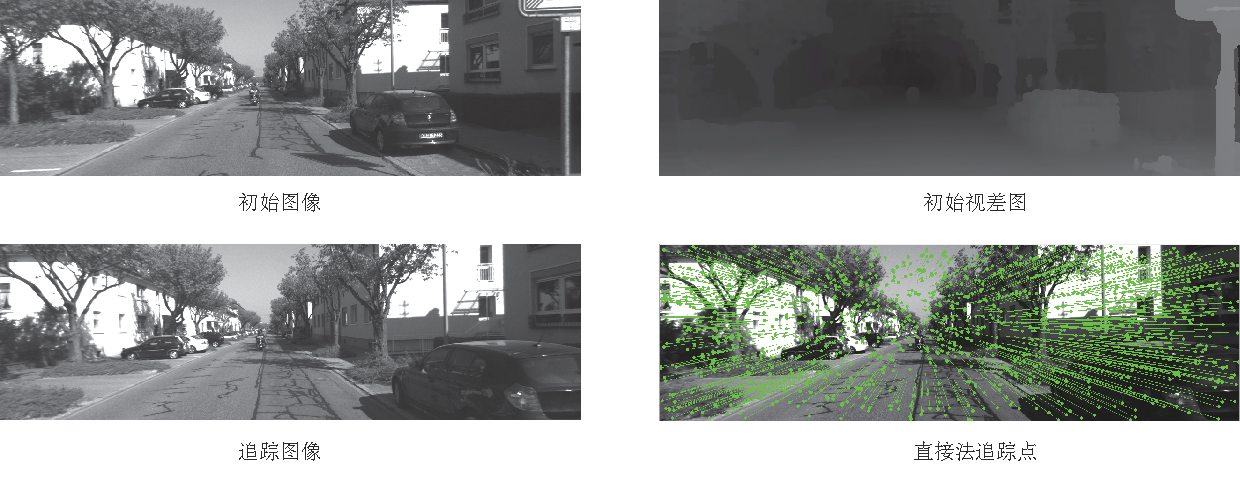
\includegraphics[width=1.0\linewidth]{vo2/direct-experiment}
	\caption{Experimental results of the direct method. upper left: original image; upper right: disparity map corresponding to the original image; lower left: fifth tracking image; lower right: tracking result}
	\label{fig:direct-experiment}
\end{figure}

Below we briefly explain the iterative process of the direct method. Compared with the feature point method, the direct method completely relies on the optimization to solve the camera pose. It can be seen from the formula \eqref{eq:jacobianofDirect} that the pixel gradient guides the direction of optimization. If you want to get the correct optimization results, you must ensure that \textbf{most pixel gradients can guide the optimization in the right direction}.

What does it mean? Assume that for the reference image, we measured a pixel with a gray value of 229. And, since we know its depth, we can infer the position of the space point $P$ (\autoref{fig:directExperiment}~shown as the grayscale measured in $I_1$).

\begin{figure}[!htp]
	\centering
	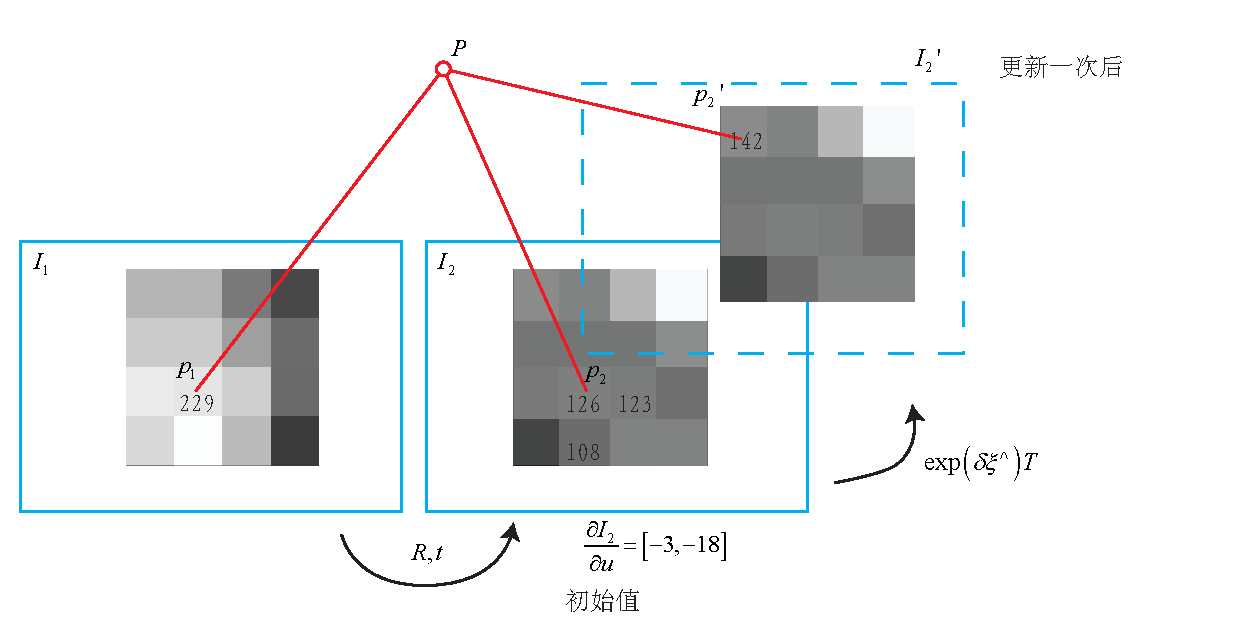
\includegraphics[width=.9\linewidth]{vo2/directExperiment}
	\caption{workflow of one iteration.}
	\label{fig:directExperiment}
\end{figure}

Now, we have got a new image and need to estimate its camera pose. This pose is obtained by continuous optimization iterations of an initial value. Assuming that our initial value is relatively poor, under this initial value, the pixel gray value after the projection of the space point $P$ is 126. Therefore, the error of this pixel is $229-126=103$. In order to reduce this error, we hope to \textbf{fine-tune the camera's pose to make the pixels brighter}.

How do I know where to fine-tune the pixels to make them brighter? This requires the use of local pixel gradients. We found in the image that if we take a step forward along the $u$ axis, the gray value at that point becomes 123, that is, 3 is subtracted. Similarly, if you take a step forward along the $v$ axis, the gray value is reduced by 18 and becomes 108. Around this pixel, we see that the gradient is $[-3,-18]$. In order to increase the brightness, we will suggest optimizing the algorithm to fine-tune the camera so that the image of $P$ moves to \textbf{top left}. In this process, we use the local gradient of the pixel to approximate the grayscale distribution near it, but please note that the real image is not smooth, so this gradient is not valid at a distance.

However, the optimization can't just follow the behavior of just one pixel, but also need to get track of other pixels. After considering many pixels, the optimization algorithm chose a place not far from the direction we suggested, and calculated an update amount $\exp ({\mathbf{\xi}^\wedge} )$. After adding the update amount, the image has moved from $I_2$ to $I_2'$, and the projection position of the pixel has also changed to a brighter place. We see that with this update, \textbf{error has become smaller}. Under ideal circumstances, we expect the error to continue to decrease and eventually converge.

But is this actually the case? Do we really only need to walk along the gradient direction to reach an optimal value? Note that the gradient of the direct method is directly determined by the image gradient, so we must ensure that \textbf{when walking along the image gradient, the photometric error will continue to decrease}. However, the image is usually a very strong \textbf{non-convex function}, as shown in \autoref{fig:non-convex}~. In practice, if we move along the image gradient, it is easy to fall into a local minimum due to the non-convexity (or noise) of the image itself, and we cannot continue to optimize. The direct method can only be established when the camera movement is very small and the gradient in the image will not have strong non-convexity.

\begin{figure}[!htp]
	\centering
	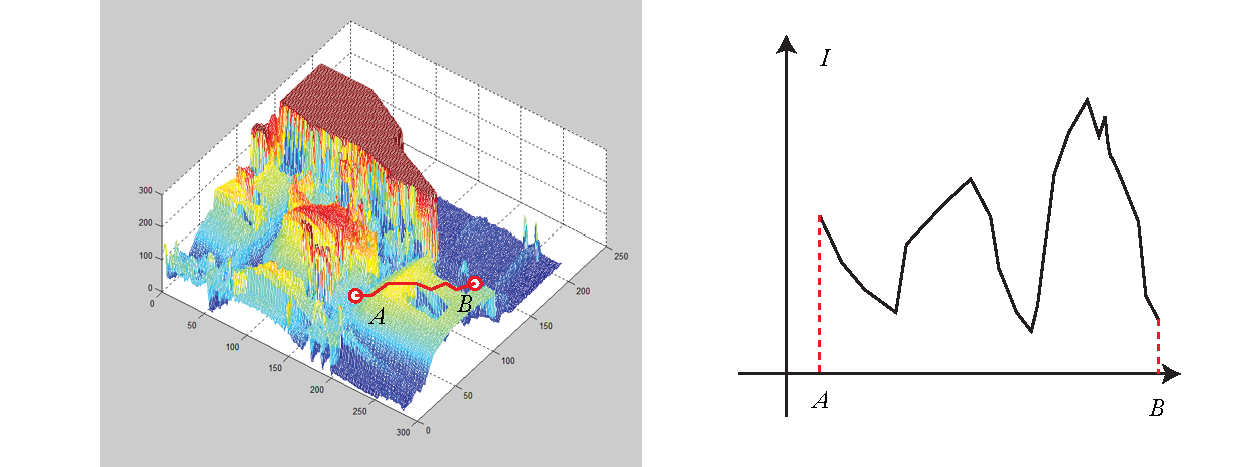
\includegraphics[width=1.0\linewidth]{vo2/nonconvex}
	\caption{Three-dimensional visualization of an image. The path from one point in the image to another point is not necessarily a "straight downhill road", but needs to be "climbing over the mountains" frequently. This reflects the non-convexity of the image itself.}
	\label{fig:non-convex}
\end{figure}

In the example, we only calculated the difference of a single pixel, and this difference is obtained by directly subtracting the grayscale. However, a single pixel is not distinguishable, and there are probably many pixels around with similar brightness. Therefore, we sometimes use small patches and use more complex difference measures, such as Normalized Cross Correlation (NCC). For the sake of simplicity, the example uses the sum of squares of errors to maintain consistency with the derivation.

\subsection{Advantages and disadvantages of the direct method}
Finally, we summarize the advantages and disadvantages of the direct method. In general, its advantages are as follows:

\begin{itemize}
	\item It can save the time of calculating feature points and descriptors.
	\item Only pixel gradients are required, no feature points are required. Therefore, the direct method can be used in the absence of features. An extreme example is an image with only gradients. It may not be able to extract corner features, but its motion can be estimated by a direct method. In the demonstration experiment, we see that the direct method can also work normally for randomly selected points. This is very important in practice, because practical scenes may not have many corner points to use.。
	\item It is possible to construct semi-dense or even dense maps, which cannot be achieved by the feature point method.
\end{itemize}

On the other hand, its shortcomings are also obvious:
\begin{itemize}
	\item \textbf{Non-convexity}. The direct method completely relies on gradient search and reduces the objective function to calculate the camera pose. The objective function needs to take the gray value of the pixel, and the image is a strongly non-convex function. This makes the optimization algorithm easy to be stuck at a local minimum, and the direct method can only succeed when the movement is small. Against this, the pyramids can reduce the impact of non-convexity to a certain extent.
	\item \textbf{Single pixel has no discriminativeness}. Many points look alike. So we either calculate image patches or calculate complex correlations. Since each pixel has inconsistent "opinions" about changing the camera movement, only a few obey the majority, and increasing the quantity for better quality. Therefore, the performance of the direct method decreases significantly when there are fewer selected points. We usually recommend using more than 500 points.
	\textbf{Brightness constant is a strong assumption}. If the camera is automatically exposed, when it adjusts the exposure parameters, it will make the overall image brighter or darker. This situation also occurs when the light changes. The feature point method has a certain tolerance to illumination, while the direct method calculates the difference of brightness, and the overall brightness change will destroy the brightness constant assumption and make the algorithm fail. In response to this, the practical direct method will also estimate the camera's exposure parameters \cite{Engel2016} so that it can still work when the exposure time changes.
\end{itemize}

\section*{习题}
\begin{enumerate}
	\item In addition to LK optical flow, do you know other optical flow methods? What are their characteristics?
	\item In the program to calculate the image gradient, we simply calculate the difference between the brighteness of $u+1$ and $u-1$ divided by 2 as the gradient in the direction of $u$. What are the disadvantages of this approach? Hint: For features closer together, the changes should be faster; while for features farther away it changes more slowly in the image, can this information be used when calculating the gradient?
	\item Can the direct method be implemented in an "inverse" way like optical flow? That is, use the gradient of the original image instead of the gradient of the target image?
	\item[\optional] Use Ceres or g2o to implement sparse direct method and semi-dense direct method.
	\item Compared with the direct method of RGB-D, the monocular direct method is often more complicated. In addition to the unknown matching, the pixel distance is also to be estimated, and we need to use the pixel depth as an optimization variable during optimization. Refer to the literature \cite{Engel2013, Engel2014}, can you understand its principle?
\end{enumerate}


